\section{Examples of path iterators}
\label{app:pathIteratorExamples}
%-----------------
%K-PATH EXAMPLE
%-----------------
\begin{figure}[ht]
\begin{subfigure}{.5\textwidth}
  \centering
  % include first image
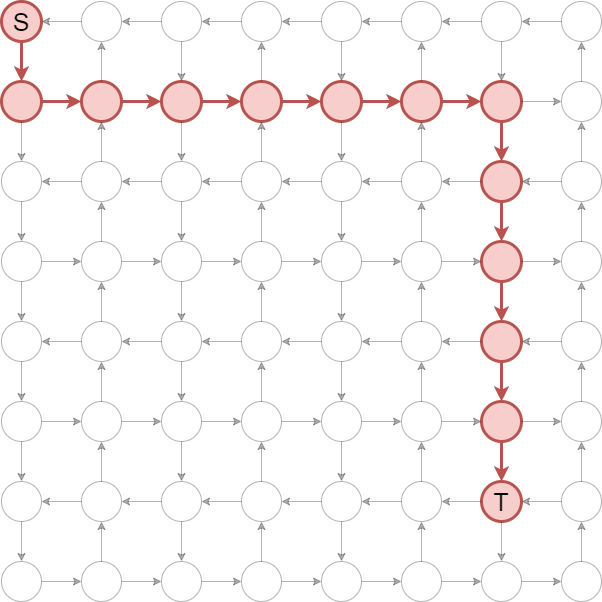
\includegraphics[width=0.8\linewidth]{images/pathiterators/examples-kpath-1.png}
  \caption{First path}
\end{subfigure}
\begin{subfigure}{.5\textwidth}
  \centering
  % include second image
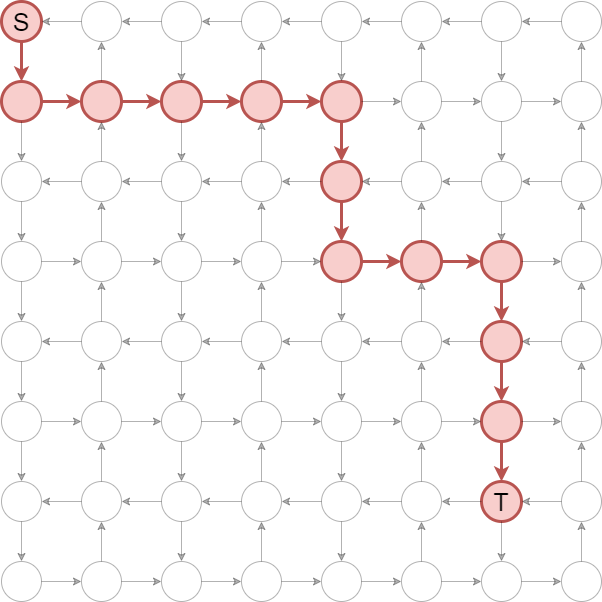
\includegraphics[width=0.8\linewidth]{images/pathiterators/examples-kpath-2.png}
  \caption{Second path}
\end{subfigure}
\caption{The first two iterations of the K-path path iterator in a square graph. This example is unaffected by ``refusing longer paths".}
\label{fig:pathexamples-kpath}
\end{figure}

%-----------------
%DFS EXAMPLE
%-----------------
\begin{figure}[ht]
\begin{subfigure}{.5\textwidth}
  \centering
  % include first image
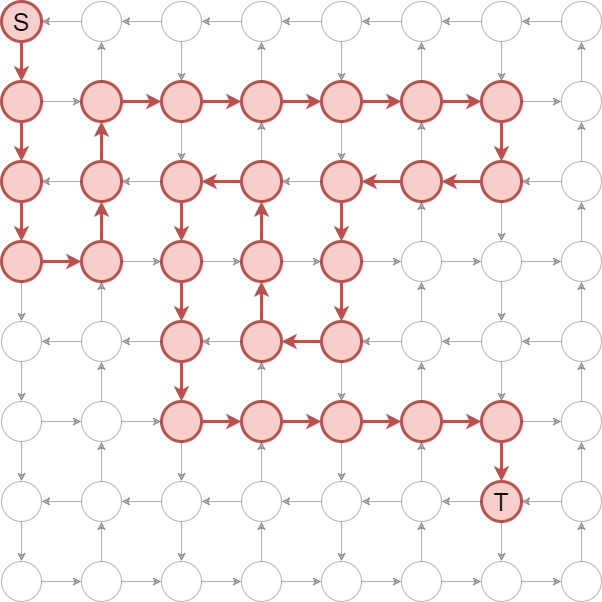
\includegraphics[width=0.8\linewidth]{images/pathiterators/examples-DFS-1.png}
  \caption{First path}
\end{subfigure}
\begin{subfigure}{.5\textwidth}
  \centering
  % include second image
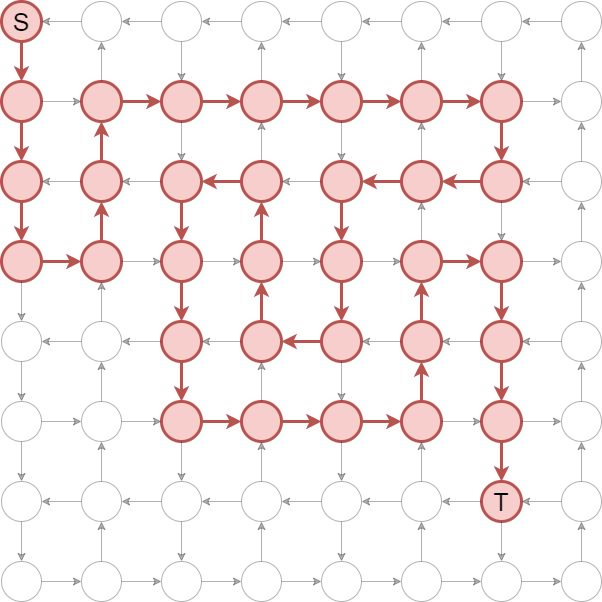
\includegraphics[width=0.8\linewidth]{images/pathiterators/examples-DFS-2.png}
  \caption{Second path}
\end{subfigure}

\begin{subfigure}{.5\textwidth}
  \centering
  % include second image
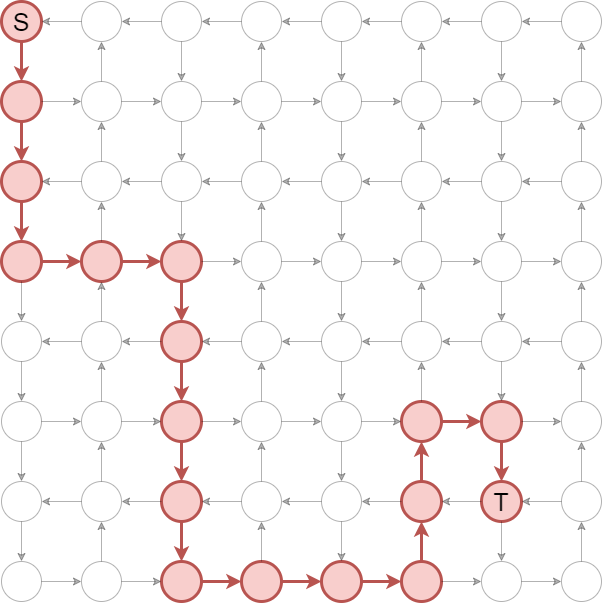
\includegraphics[width=0.8\linewidth]{images/pathiterators/examples-DFS-1-RLP.png}
  \caption{First path (refusing longer paths)}
\end{subfigure}
\begin{subfigure}{.5\textwidth}
  \centering
  % include second image
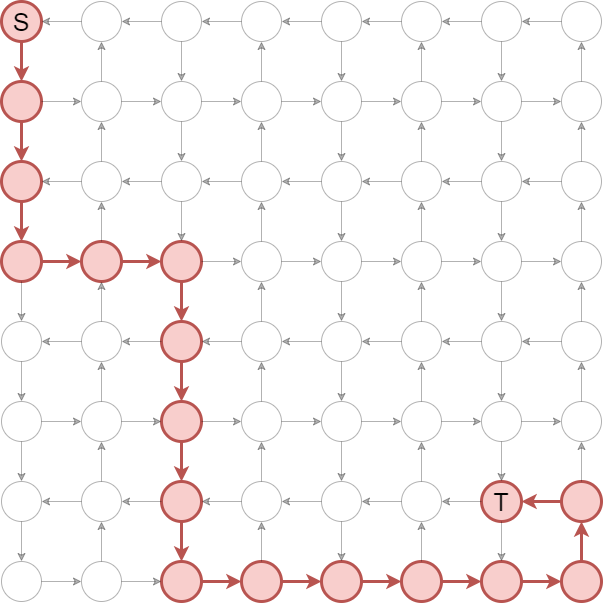
\includegraphics[width=0.8\linewidth]{images/pathiterators/examples-DFS-2-RLP.png}
  \caption{Second path (refusing longer paths)}
\end{subfigure}
\caption{The first two iterations of the DFS path iterator in a square graph.}
\label{fig:pathexamples-dfs}
\end{figure}



%-----------------
%GREEDY DFS EXAMPLE
%-----------------
\begin{figure}[ht]
\begin{subfigure}{.5\textwidth}
  \centering
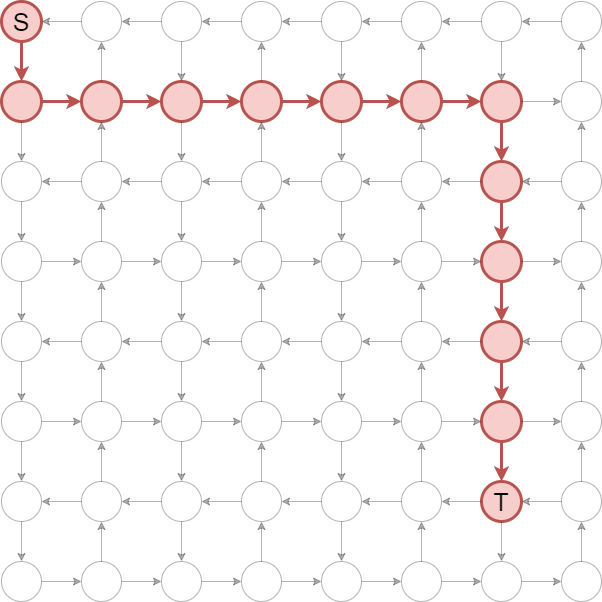
\includegraphics[width=0.8\linewidth]{images/pathiterators/examples-Greedy DFS-1.png}
  \caption{First path}
\end{subfigure}
\begin{subfigure}{.5\textwidth}
  \centering
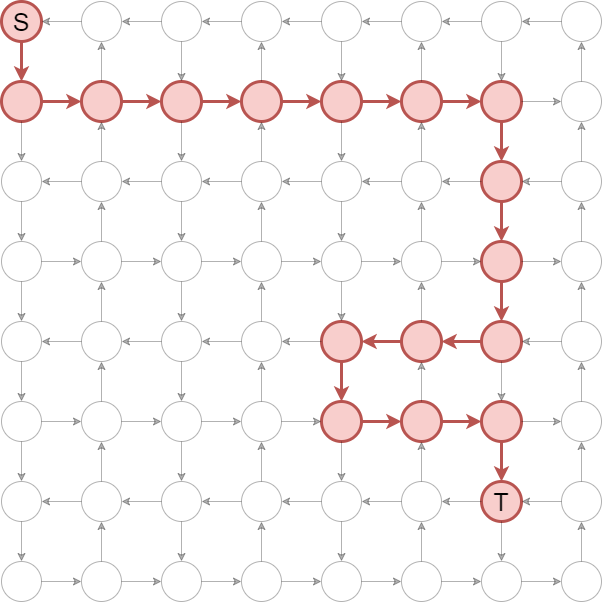
\includegraphics[width=0.8\linewidth]{images/pathiterators/examples-Greedy DFS-2.png}
  \caption{Second path}
\end{subfigure}

\begin{subfigure}{.5\textwidth}
  \centering
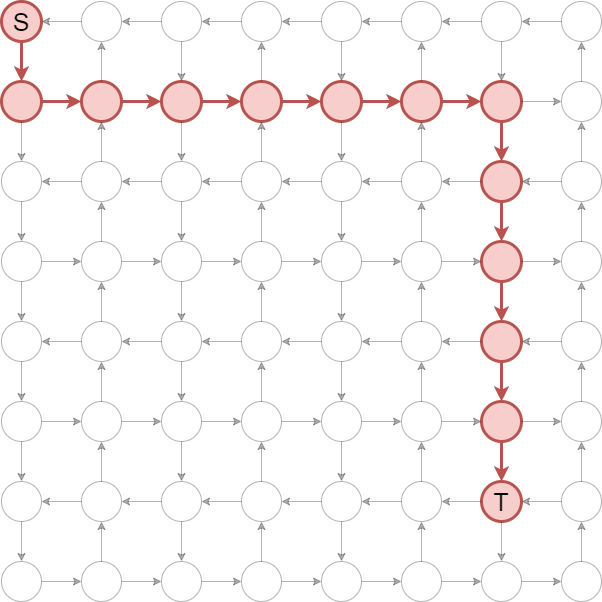
\includegraphics[width=0.8\linewidth]{images/pathiterators/examples-Greedy DFS-1.png}
  \caption{First path (refusing longer paths)}
\end{subfigure}
\begin{subfigure}{.5\textwidth}
  \centering
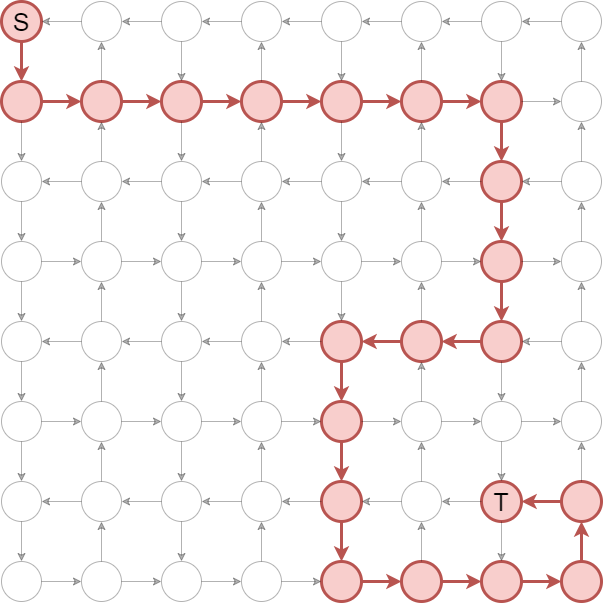
\includegraphics[width=0.8\linewidth]{images/pathiterators/examples-Greedy DFS-reflongerpaths.png}
  \caption{Second path (refusing longer paths)}
\end{subfigure}
\caption{The first two iterations of the greedy DFS path iterator in a square graph.}
\label{fig:pathexamples-greedydfs}
\end{figure}

%-----------------
%CONTROL POINT EXAMPLE
%-----------------
\begin{figure}[ht]
\begin{subfigure}{.5\textwidth}
  \centering
  % include first image
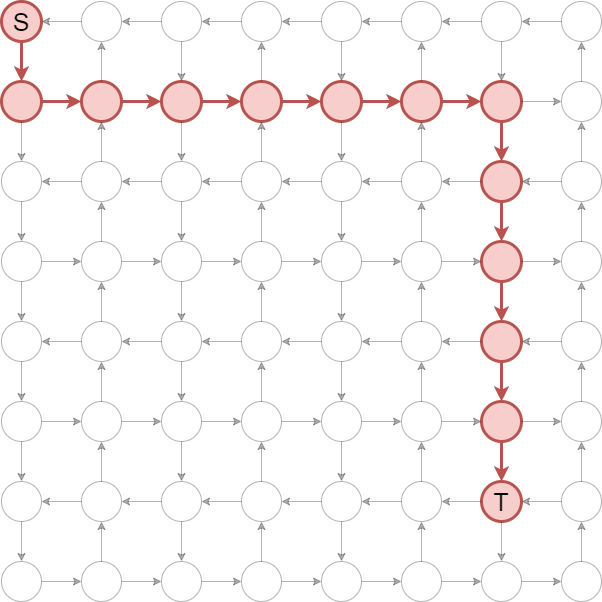
\includegraphics[width=0.8\linewidth]{images/pathiterators/examples-Control point-1.png}
  \caption{First path (0 control points)}
\end{subfigure}
\begin{subfigure}{.5\textwidth}
  \centering
  % include second image
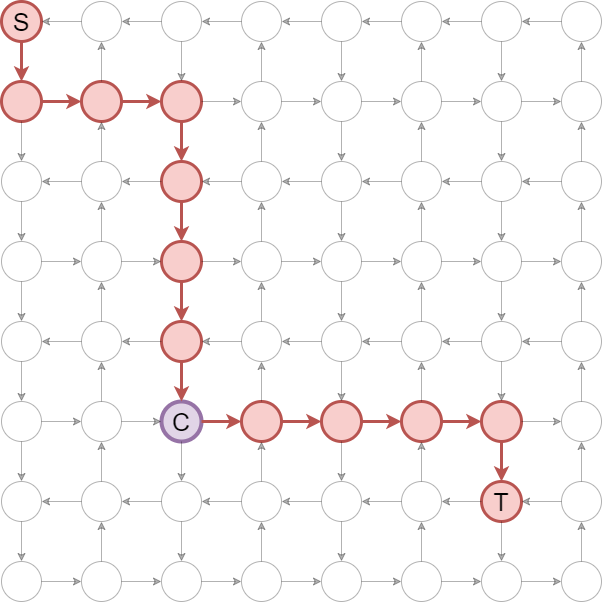
\includegraphics[width=0.8\linewidth]{images/pathiterators/examples-Control point-2.png}
  \caption{Second path (1 control point)}
\end{subfigure}
\caption{The first two iterations of the control point path iterator in a square graph. This example is unaffected by ``refusing longer paths".}
\label{fig:pathexamples-controlpoint}
\end{figure}